\documentclass[12pt]{article}
\usepackage{graphicx}
\begin{document}
\textbf{First of all, the article reads to me almost as two separate studies. 
The first one (everything up to section 4.1), about actual cloud tracking and 
the statistics thereof, suffers from being not very thorough, or at least not 
adding a lot to previous articles by the authors as well as the work by Heus et 
al. That is, the automated algorithm is an excellent achievement in itself, but 
I don't see the additional statistics being used a lot.}

\textbf{The second part of the article is the part that really shines to me.
However, one could argue that that part of the article suffers from only 
starting at page 13 of the article, thus easily overlooked. I wonder what the 
reason of the authors was to put this all together in one article.}

\vspace{5mm}

We see the first part of the article as being a description of the algorithm 
and characterization of the cloud population produced by the algorithm, and the
second part of the article as an application of this algorithm to examine a 
cloud field.  The statistics in the first section are intended to compare the
algorithm output to our understanding of cloud fields to ensure the algorithm 
is not substantially distorting the cloud statistics.  As such, the first part 
of the paper does not contain original results concerning the statistics of 
cloud fields, as that would defeat the purpose of comparing the results of the
algorithm with known cloud statistics.  The second part is original research on 
cloud field properties we use to illustrate the potential uses of our 
algorithm. We believe both parts are integral to a presentation of our
algorithm. We have detailed this rationale more clearly in the introduction to 
the paper and at other appropriate points.

\vspace{5mm}

\textbf{Shouldn't the title be ...analysis of an LES shallow....?}

\vspace{5mm}

Yes. We have altered the title, and every other occurrence of ``a LES'' in the 
text.

\vspace{5mm}

\textbf{p23235, l.14 and other places: Couvreux is spelled without the `a'}

\vspace{5mm}

We have corrected these errors.

\vspace{5mm}

\textbf{p23236, l.13: Enforcing condensed points to be a subset of the plume 
points is fine I'm sure for studies on transport, but isn't it giving a bias in 
that it neglects passive clouds?}

\vspace{5mm}

We did not intend to indicate that the condensed points must be part of the
plume to be counted as condensed, but rather that condensed points are all 
flagged as plume points as well, regardless of their tracer concentration.  
Passive clouds should be tracked by this scheme, but will be unable to split or 
merge with other clouds.  We have altered the text to read ``Finally, all
condensed points are also flagged as plume points regardless of their tracer 
concentration, so that the condensed region is always a subset of the plume.''

\vspace{5mm}

\textbf{p23236 the definition of cloudlets is not completely clear to me, and 
not always consistently used in the article, I believe. What is the difference
between clouds and cloudlets?}

\vspace{5mm}

Cloudlets are sub-divisions of contiguous clouds formed by splitting the clouds 
around contiguous areas of cloud core.  Each cloudlet has one, and only one, 
region of core points.  For example, if a cloud contains two spatially 
unconnected regions of cloud core, the cloud will be divided into two 
cloudlets, each formed around one of the core regions.  We have added a clearer
explanation of this to section 3.1.

\vspace{5mm}

\textbf{p23236, l.21: How is a split cloudlet being divided over 2 cloudlets,
exactly? I assume by some proximity to the center or mass, or something like 
that, but this is not clear.}

\vspace{5mm}

Clouds are split into cloudlets by proximity to core regions inside the clouds. 
We have rewritten the tracking description to try to make this clearer.

\vspace{5mm}

\textbf{p23237, second and third paragraph: This is a rather technical 
discussion, that could benefit from a better graphicial depiction. All actions 
should be depicted in some sense (and cross referenced between the figure and 
the text). Also, from figure 2 it isn’t clear to me what the difference between 
cloud 2/3 and 4 really is. Given that the description of the algorithm is an
important goal of the paper, more care to clarity here is necessary.}

\vspace{5mm}

%TK

\vspace{5mm}

\textbf{p23238 The implicit definition that Zhao\&Austin, and Heus et al, 
used for a cloud is a connected area in space and time that emerges and decays 
within the window of observation, including the entire lineage of splitting and
merging 'cloudlets'. That means that many of your 3171 do not qualify as such,
because they either are involved in splitting and merging events, or have a 
lifespan that reaches over the boundaries of the observation window. So: How 
many clouds according that definition are actually tracked? How long does the
tracking algorithm need in terms of CPU time? This is relevant because you 
claim to have significantly better statistics with less human effort. So how 
does this compare to the tens of clouds selected by Heus et al, in a process 
that took maybe a few days of cherry picking?}

\vspace{5mm}

If we do not allow splits and ignore all clouds that are present at the start 
and end of the simulation, we end up with 1678 clouds.  However, tracking the 
cloud field in this manner means that fleeting connections between two clouds 
result in disconnected condensed regions being considered to be a single cloud, 
no matter how long since they have been connected or how brief the connection.  
This profoundly biases the sample, as the majority (well over 50\%) of the 
cloud field area becomes connected into less than 10 large 'clouds' which are 
not spatially localized (parts of the 'clouds' are on opposite sides of the 
domain), and which are present at either the start or end of the data period. 
The longest-lived cloud persists for the entire 3-hour duration of the model 
output, and at its peak represents about 45\% of the total cloud base area.
Unconnected clouds of the type described by Heus et al. 2009 appear to be the
exception rather than the rule--or at least, they are in the System for 
Atmospheric Modeling LES of BOMEX.  We have added an explanation of this result 
to the start of section 3 to help motivate the creation of this algorithm.

Additionally, unlike Heus et al., our technique does not require use of a 
Virtual Reality environment or other specialized equipment, and removes 
possible human selection biases from the cloud sample.  We believe these are
significant advantages for our technique.

Our algorithm takes 1 hour and 40 minutes to process the BOMEX LES output as a 
single-threaded process running on an Intel Xeon E5645 2.4 GHz processor with 
4 GB of RAM. We have added this informtion to the cloud tracking results.

\vspace{5mm}

\textbf{p23239/Figure 3: This cloud worries me a bit. Its cloud fraction at 
cloud base seems to be close to 1 percent, that is: Close to the entire cloud 
field of BOMEX. It also has a duration that is a big part of the measurement 
window. How dominating is this cloud within the sample?}

\vspace{5mm}

The total BOMEX cloud fraction at cloud base in our model is about 0.065, 
in reasonable agreement with the lower resolution models used in the original
BOMEX LES comparison (Siebesma et al. 2003).  This cloud thus represents over 
10\% of the total cloud base area at times.  We have added a brief discussion
of the relative size of this cloud to our description of the cloud tracking 
results section 3.2. 

As we mention in this response above, neglecting splits results in the largest 
cloud occupying 45\% of the total cloud base area. Comparing our cloud tracking 
area distribution with one calculated from instantaneous snapshots (as shown in
Figure 6 of the paper) indicates that our algorithm greatly reduces the number 
of clouds with $a^{1/2} > 1000$ metres. This suggests that our algorithm makes 
the clouds too small, rather than too large.  As for the apparent dominance of 
large clouds versus small clouds in the BOMEX cloud field, we feel this subject 
is outside the scope of this article, and intend on addressing this question in 
our next publication.

\vspace{5mm}

\textbf{p23240/Fig 5: What are the bin widths? This is important here to 
understand what the relative numbers are.}

\vspace{5mm}

The bin widths used in Figure 5 are: a) 2 minutes, b) 10$^6$ kg, c) 50 m and 
d) 50 m.  We have added this information to the Figure 5 caption.

\vspace{5mm}

\textbf{p23240/Fig 5: This is a figure that with the tracking algorithm in 
place, a lot more can be done with. For instance, your figure 1 shows that some 
cloud bases rise at the end of their life time, but not all. A 2D pdf of Cloud 
base and Cloud height vs relative cloud life time would be more interesting to 
me than these plots (c and d at least), that are not all that different from 
what can be done without tracking.}

\vspace{5mm}

Again, the point of these plots is not to present new results, but to establish 
exactly how our algorithm affects the cloud statistics.  As such, we feel that 
presenting novel results in this section would be counter-productive.

\vspace{5mm}

\textbf{p23241: If I understand this right, the cloud size distribution is 
still an instantaneous property, merely to validate your cloud sample as 
something that is a realistic reflection of the entire cloud field. I’d be 
interested to see a discussion here on the role of the lifecycle in skewing the 
cloud size distribution. I could imagine that taking the lifecycle average 
cloud size has a similar effect: Small clouds may become bigger later in their 
life time, and large clouds have on average a smaller size during their 
lifetime. So what does the distibution look like for average and/or maximum 
cloud size over its lifetime?}

\vspace{5mm}

Figure 5b) in our paper is a reasonable proxy for the distribution of average 
cloud size.  It appears to remain a power law relationship.  However, since 
the largest clouds also tend to be the longest-lived, there will be fewer 
large clouds in a distribution of average or maximum cloud size clouds, making 
the power law slope steeper for `lifetime' versus `instantaneous' distributions.

Again, we feel that such a discussion is extraneous to the point of this 
section, which is to characterize the output of our algorithm by examining how 
it modifies more traditional measures of cloud field statistics.

\vspace{5mm}

\textbf{p23242: Like with for example Neggers, a scale brake at 1 km is not all 
that surprising, given that your domain is only 6.4 km wide. And while your 
$\lambda$ agrees well with the literature, a range between 1.7 and 2.3 is a 
fairly big range. Does your study shed some light on what could be the reason 
for the differences between the various studies? Does the air plane bias 
towards older clouds (one can’t aim for clouds that haven’t popped up yet) or 
the 2D bias of satellite observations play a role here?}

\vspace{5mm}

We have not analysed our data in a manner that would shed light on these issues,
though our technique could likely be used to address them.  Without such an 
analysis, we are hesitant to comment on this subject.

\vspace{5mm}

\textbf{p23243/ Fig 7: I assume these correlations are on the in cloud minus 
slab averaged values? Otherwise, strong correlations are perhaps not so 
surprising.}

\vspace{5mm}

This should not matter, since the definition of correlation involves removing 
the mean from each variable being correlated.

\vspace{5mm}

\textbf{p23243: It is interesting to see the strong correlation between $M$ 
and $a$, in contrast with the small correlation between $w$ and $a$. Can the 
authors comment on that a bit more?}

\vspace{5mm}

This results from the power law distribution of cloud areas.  We have added the
following paragraph to section 4: 

``Although $M$ is related to $a$ and $w$ via the relation $M = \rho w a$, where 
$\rho$ is the air density in kg m$^{-3}$, $M$ is only weakly correlated with 
$w$, despite being strongly correlated with $a$.  This unintuitive result 
arises due to the relative contributions of $a$ and $w$ to the variance of $M$.
Changes in $M$ can be expressed in terms of changes in $a$ and $w$ as
\begin{equation}
\label{eq:Mpartials}
d M = \rho w \partial {a} + \rho a \partial {w}
\end{equation}
Choosing representative cloud layer values into (\ref{eq:Mpartials}) is 
complicated by the power-law distribution that governs cloud areas.  The median 
values of $w$ and $a$ are roughly 0.5 m s$^{-1}$ and 10000 m$^2$ (Figure 8), 
while 66\% of $w$ and $a$ fall between roughly (0.1-1.0) m s$^{-1}$ and
(1000-100000) m$^{2}$, respectively.  Differences in cloud vertical velocity 
will thus result in mass flux values of approximately (1000-10000) kg s$^{-1}$, 
while differences in cloud cross-sectional area will results in mass flux 
values between (500-50000) kg s$^{-1}$, a range an order of magnitude larger.  
Thus, cloud mass fluxes are primarily controlled by the area of the cloud, 
producing near unity correlations between $a$ and $M$.''

\vspace{5mm}

\textbf{p23246: An interesting extension of Romps indeed. Especially the 
correlation in dynamics, but the lack thereof in thermodynamic quantities is
interesting. A 'nature-like' approach would suggest that big area cloud bases 
would result in less entrainment/detrainment (as shown by Fig 12), which would
maintain the cloud. If sample size allow it, it would be interesting to see 
whether there is a bit more of a spatial correlation in $q_t$ if looking at 
only the biggest cloud (bases).}

\vspace{5mm}

Eliminating small cloud base area (less than 50000 m$^2$--about 80 grid cells) 
clouds increases the correlation between upper-level buoyancy and cloud base 
velocity slightly (Figure (1)), but other variables actually show reduced 
correlations.  This is because cloud base properties are fairly uniform and so 
do not have a large dynamic range with which to correlate with upper-level 
properties.  Removing small area clouds actually serves to reduce the dynamic 
range of the cloud base variables, reducing upper-level predictability.

\begin{figure}[t]
\begin{center}
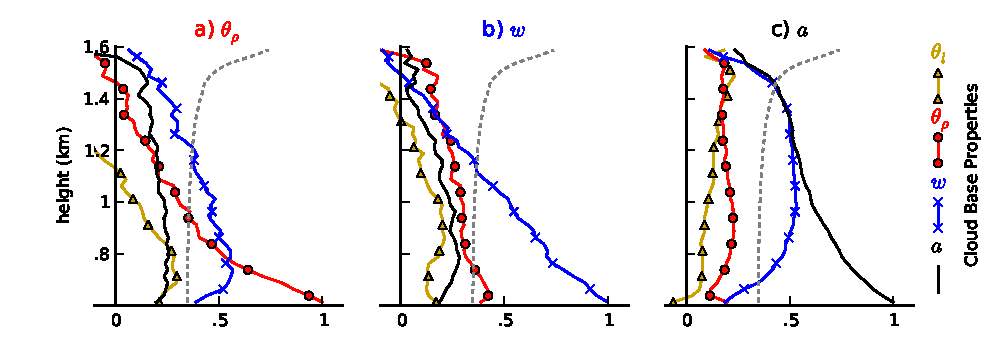
\includegraphics[width=\textwidth]{cloud_base_profiles_nosmall.eps}
\end{center}
\caption{Correlation profiles between cloud base properties at 600m and at 
higher levels, with cloud base areas \textless 50000 m$^2$ removed from the 
sample.}
\end{figure}

\vspace{5mm}

\textbf{p23247/Fig13: What is the added value of this plot? I would at least 
plot the domain averaged $q_t$ to get a feeling for the deviation there.}

\vspace{5mm}

This plot provides direct evidence to show that larger clouds shield their 
interiors from the effects of entrainment, and so parcel models should take 
cloud area into account when calculating entrainment rates.

We have added the domain averaged $q_t$ to the plot.

\vspace{5mm}

\textbf{Table 1: This table contains a lot of information, but it is not 
always immediately clear where to look. A color/grey background for the 
significant ones could help a lot already. Also, the headers are a bit 
cryptic.}

\vspace{5mm}

We have added a grey background to the significant entries in the table, and 
have attempted to make the headers clearer. 

\vspace{5mm}

\end{document}
